\section{RCRRTBall\-Dual  Class Reference}
\label{classRCRRTBallDual}\index{RCRRTBallDual@{RCRRTBall\-Dual}}
Basic dual tree version of {\bf RCRRTBall} {\rm (p.\,\pageref{classRCRRTBall})}. 


{\tt \#include $<$rcrrt.h$>$}

Inheritance diagram for RCRRTBall\-Dual::\begin{figure}[H]
\begin{center}
\leavevmode
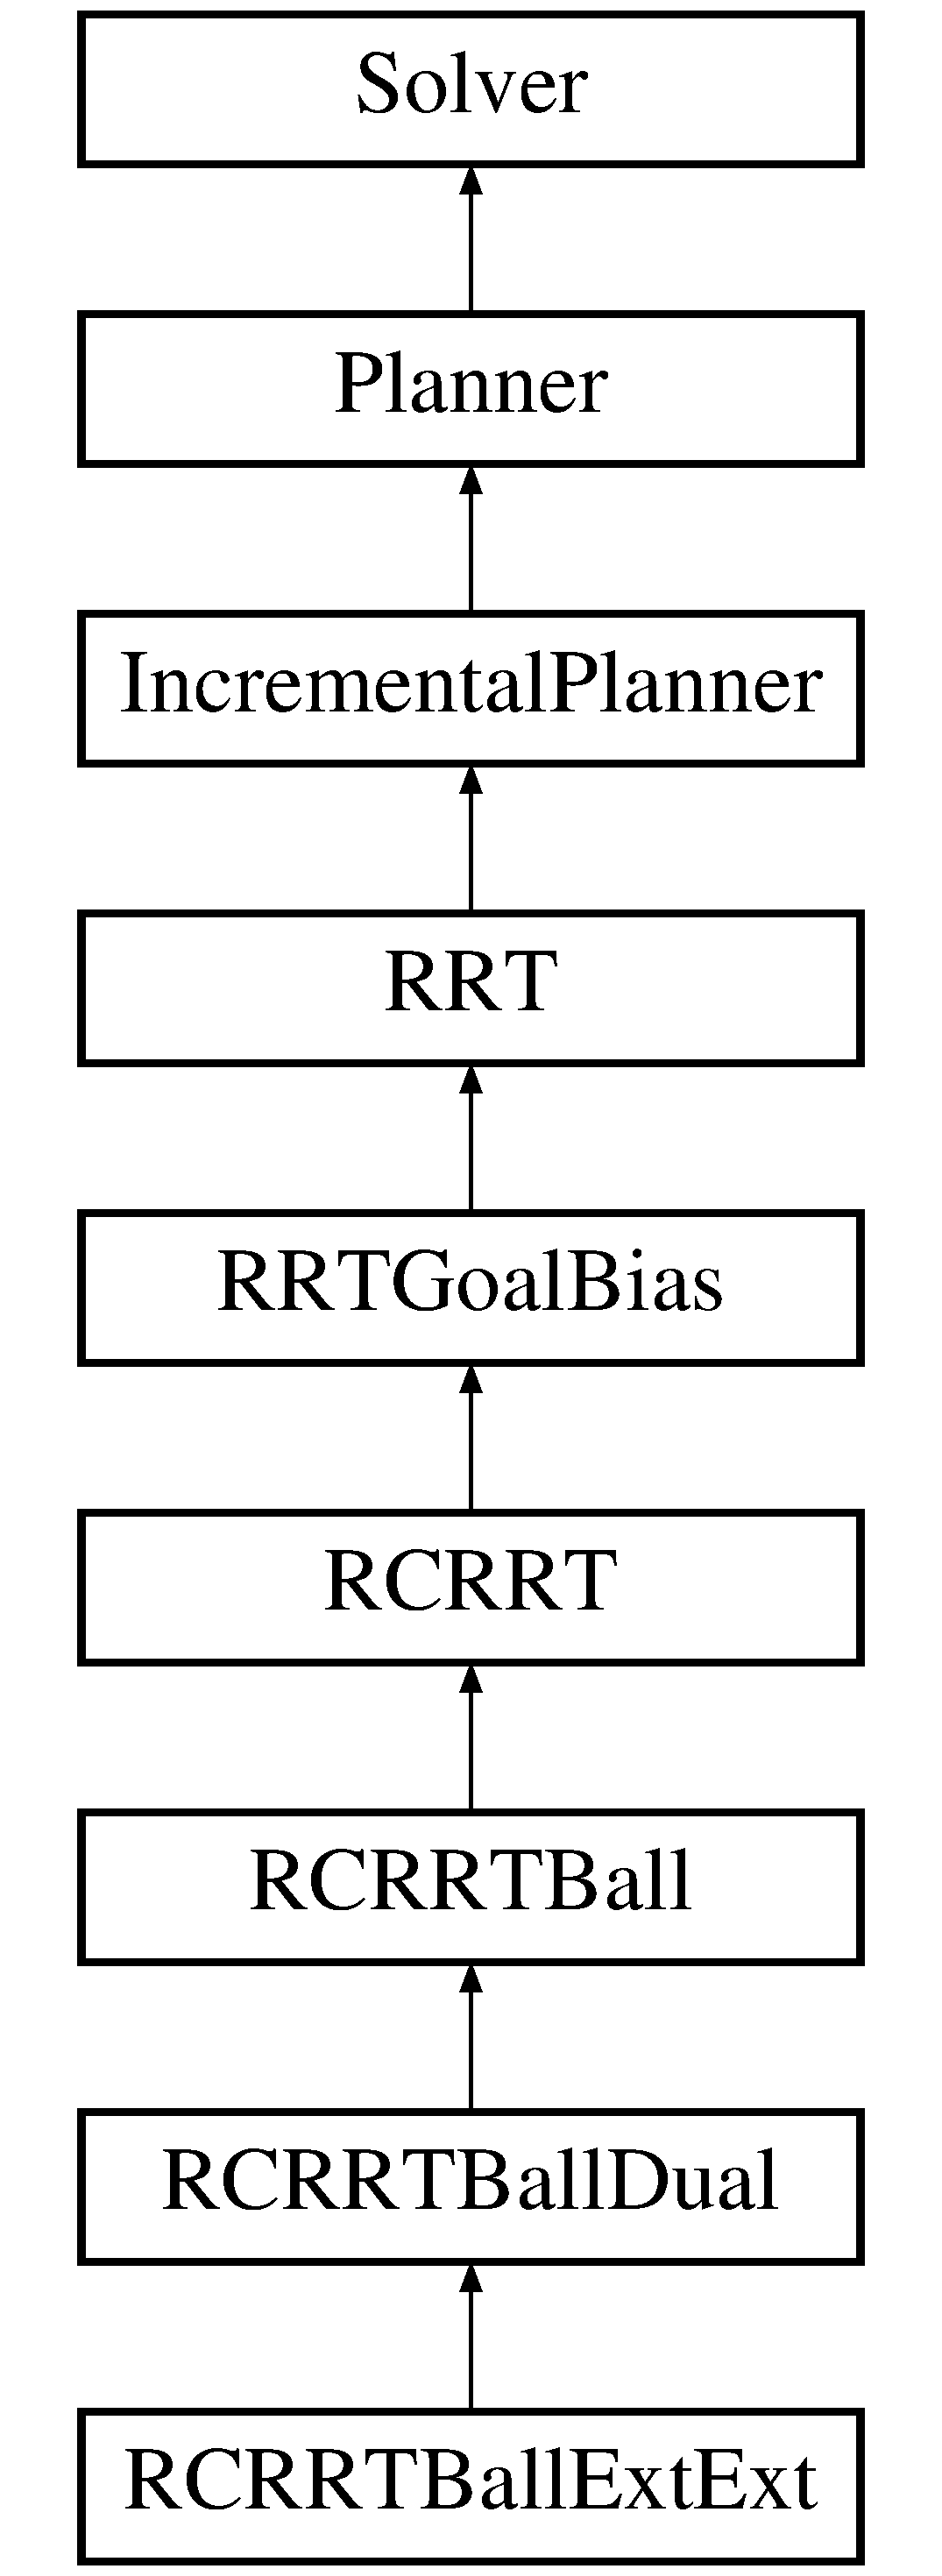
\includegraphics[height=9cm]{classRCRRTBallDual}
\end{center}
\end{figure}
\subsection*{Public Methods}
\begin{CompactItemize}
\item 
{\bf RCRRTBall\-Dual} ({\bf Problem} $\ast$p)
\item 
virtual {\bf $\sim$RCRRTBall\-Dual} ()
\item 
virtual bool {\bf Plan} ()
\begin{CompactList}\small\item\em Attempt to solve an Initial-Goal query by growing an {\bf RRT} {\rm (p.\,\pageref{classRRT})}.\item\end{CompactList}\item 
virtual bool {\bf Get\-Connected} ({\bf MSLNode} $\ast$n1, {\bf MSLNode} $\ast$n2)
\end{CompactItemize}
\subsection*{Protected Methods}
\begin{CompactItemize}
\item 
void {\bf Recover\-Solution} ({\bf MSLNode} $\ast$n1, {\bf MSLNode} $\ast$n2)
\end{CompactItemize}


\subsection{Detailed Description}
Basic dual tree version of {\bf RCRRTBall} {\rm (p.\,\pageref{classRCRRTBall})}.



\subsection{Constructor \& Destructor Documentation}
\index{RCRRTBallDual@{RCRRTBall\-Dual}!RCRRTBallDual@{RCRRTBallDual}}
\index{RCRRTBallDual@{RCRRTBallDual}!RCRRTBallDual@{RCRRTBall\-Dual}}
\subsubsection{\setlength{\rightskip}{0pt plus 5cm}RCRRTBall\-Dual::RCRRTBall\-Dual ({\bf Problem} $\ast$ {\em p})}\label{classRCRRTBallDual_a0}


\index{RCRRTBallDual@{RCRRTBall\-Dual}!~RCRRTBallDual@{$\sim$RCRRTBallDual}}
\index{~RCRRTBallDual@{$\sim$RCRRTBallDual}!RCRRTBallDual@{RCRRTBall\-Dual}}
\subsubsection{\setlength{\rightskip}{0pt plus 5cm}virtual RCRRTBall\-Dual::$\sim$RCRRTBall\-Dual ()\hspace{0.3cm}{\tt  [inline, virtual]}}\label{classRCRRTBallDual_a1}




\subsection{Member Function Documentation}
\index{RCRRTBallDual@{RCRRTBall\-Dual}!GetConnected@{GetConnected}}
\index{GetConnected@{GetConnected}!RCRRTBallDual@{RCRRTBall\-Dual}}
\subsubsection{\setlength{\rightskip}{0pt plus 5cm}bool RCRRTBall\-Dual::Get\-Connected ({\bf MSLNode} $\ast$ {\em n1}, {\bf MSLNode} $\ast$ {\em n2})\hspace{0.3cm}{\tt  [virtual]}}\label{classRCRRTBallDual_a3}


\index{RCRRTBallDual@{RCRRTBall\-Dual}!Plan@{Plan}}
\index{Plan@{Plan}!RCRRTBallDual@{RCRRTBall\-Dual}}
\subsubsection{\setlength{\rightskip}{0pt plus 5cm}bool RCRRTBall\-Dual::Plan ()\hspace{0.3cm}{\tt  [virtual]}}\label{classRCRRTBallDual_a2}


Attempt to solve an Initial-Goal query by growing an {\bf RRT} {\rm (p.\,\pageref{classRRT})}.



Reimplemented from {\bf RCRRTBall} {\rm (p.\,\pageref{classRCRRTBall_a5})}.

Reimplemented in {\bf RCRRTBall\-Ext\-Ext} {\rm (p.\,\pageref{classRCRRTBallExtExt_a2})}.\index{RCRRTBallDual@{RCRRTBall\-Dual}!RecoverSolution@{RecoverSolution}}
\index{RecoverSolution@{RecoverSolution}!RCRRTBallDual@{RCRRTBall\-Dual}}
\subsubsection{\setlength{\rightskip}{0pt plus 5cm}void RCRRTBall\-Dual::Recover\-Solution ({\bf MSLNode} $\ast$ {\em n1}, {\bf MSLNode} $\ast$ {\em n2})\hspace{0.3cm}{\tt  [protected]}}\label{classRCRRTBallDual_b0}




The documentation for this class was generated from the following files:\begin{CompactItemize}
\item 
{\bf rcrrt.h}\item 
{\bf rcrrt.C}\end{CompactItemize}
